\section[Využití detektorů v metrologii aktivity]{Využití proporcionálních detektorů a kapalných scintilátorů v metrologii aktivity radionuklidů}

Metrologie radioaktivity radionuklidů je dělena do dvou základních skupin:

\begin{itemize}
    \item Absolutní = Využívá přímé detekce veličiny (Koincidenční metoda, elektrostatická metoda, kalorimetrická metoda, absolutní počítání částic).
    \item Relativní = Vztah mezi veličinou indikovanou a veličinou měřenou (spektrometrie gama, ionizační komora).
\end{itemize}

\subsection{Využití proporcionálních detektorů}

Jedná se o primární metodu měření = vychází z definice veličiny.

Proporcionální detektor je často válcové geometrie a skládá se z anody (tenký drátek z W, Mo, Cu, ocel, Au pokrytí) a katody (tělo detektoru). Díky velkému rozdílu ve velikosti elektrod je mezi nimi velký rozdíl napětí, a to vytváří velmi intenzivní elektrické pole. Pracovním plynem uvnitř detektoru je často Ar, Kr, Xe + zhášecí plyn, což je například Metan nebo propanbutan.

Výstupní impuls na detektoru je úměrný deponované energii. Typická náplň je plyn P-10 (90\% Ar a 10\% CH$_4$).

Důležité je, aby anodový drátek měl konst. průměr a tloušťku. Výhodou proporcionálního detektoru je, že téměř nemá mrtvou dobu a je tedy hodně dobře schopen detekovat dva signály "naráz".

Je provozován v oblasti proporcionality VA charakteristiky plynového detektoru, kdy měřená četnost téměř nezávisí na napětí (pracovní napětí detektoru je zvoleno v této oblasti). Provoz v této oblasti umožňuje rozvoj townsendovy laviny, jež představuje plynové zesílení.

Plynová naplň v detektoru je přítomna za účelem zesílení vstupního signálu = plynové zesílení. Proto je proporcionální počítač vhodný pro detekci záření malých energií, které je pak třeba zesílit právě přítomným plynem (ionizace plynu k zesílení vstupního signálu, a to řádové E2 až E3).

Proporcionální počítač se používá k měření $\alpha$ a $\beta$ záření.

Proporcionální počítače lze využít jako prosté detektory čítání, ale také částečně pro spektrometrii/spektroskopii neboť výstupní signál je úměrný vstupnímu, resp. deponované energii (s uvážením zesílení od plynu).

\textbf{Druhy proporcionálních počítačů:}

\begin{itemize}

    \item Průtokový: 

        \begin{itemize}
            \item Pracovní plyn protéká detektorem o atmosférickém tlaku a díky tomu je snadná výměna vzorků.
            \item Měření $\alpha$ a $\beta$ záření, zejména pak $\beta$.
            \item Lze udělat i 4$\pi$ variantu.
            \item Vhodný pro měření nízkoenergetické $\beta$ a plynných radioaktivních sloučenin i neutronů (pro neutrony je potřeba konverzní materiál).
        \end{itemize}
    
    \item Tlakový: 

        \begin{itemize}
            \item Plynová náplň má vyšší hmotnostní číslo a plyn je natlakován do cca 1,5 MPa.
            \item Vyšší tlak umožňuje dosáhnout vyšší účinnosti detekce záření (Tím, že je to natlakované, tak se tam vejde více plynu a tím se mi zvyšuje pravděpodobnost interakce záření s plynem).
        \end{itemize}

\end{itemize}


\textbf{Korekce:}

Zejména pro interní proporcionální poćítač, kdy je měřený vzorek uvnitř.

\begin{itemize}
    \item Koncový efekt = Na okrajích elektrod je elektrické pole deformované. Lze kompenzovat využitím dvou počítačů různé délky a rozdíl odezvy odpovídá četnosti naměřené ideálním detektorem o délce rozdílu jejich délek.
    \item Stěnový efekt = částice emitovaná v blízkosti stěn nestačí dostatečně ionizovat (oprava na základě měření s několika počítači stejné délky různých poloměrů, vliv klesá s rostoucím tlakem plynové náplně)
\end{itemize}

\subsection{Využití kapalných scintilátorů}

Jedná se o scintilační detektor, kde scintilační látka je tekutá/roztok. Jedná se o roztoky scintilačních látek v organických rozpouštědlech + měřený vzorek, který je v tomto taktéž rozpuštěn (podle druhu měřeného vzorku se používají rozpouštědla jako je toulen, xylen, ethalon).

Kapalné scintilátory se používají pro detekci IZ ($\alpha$ a $\beta$) o vyšších energiích (minimální detekovatelná energie je 3-10 keV). Využívají se pro tzv. metodu TDCR (triple to double coincidence ratio).

Detekční účinnost je dána účinnosti fotokatody daného fotonásobiče (kvalita fotonásobiče).

\subsubsection{TDCR}

Jedná se o koincidenční zapojení tří fotonásobičů, jež funguje na principu poměru trojných a dvojných koincidencí. Tato metoda slouží ke stanovení počítací účinnosti, a to experimentálně bez potřeby kalibračního standardu.

počítací účinnost ($\varepsilon_D$), neboli parametr TDCR (v zásadě detekční účinnost) se určuje na základě srovnání experimentu a modelu $\rightarrow$ v praxi je měřeno TDCR pro různé účinnosti detekce, které mohu měnit defokusací PMT, optickými filtry atd. Tím získávám závislost naměřené aktivity na TDCR (aktivita by měla být nezávislá na TDCR - kritérium správnosti) a dále závislost detekční účinnosti na TDCR (tu detekční účinnost si měním). Ve výsledku srovnáním experimentu a modelu získám účinnost $\varepsilon_D$:

$$ \left( \frac{\varepsilon_T}{\varepsilon_D} \right)_\text{výpočet} = \left( \frac{N_T}{N_D} \right)_\text{měření}. $$

Výsledný počet řešení TDCR parametru se odvíjí od druhu radionuklidu a složitosti jeho kaskády rozpadu.

Výsledná aktivita je získána jako: 

$$ A = \frac{N_D}{\varepsilon_D}. $$

\begin{figure}[ht!]
    \centering
    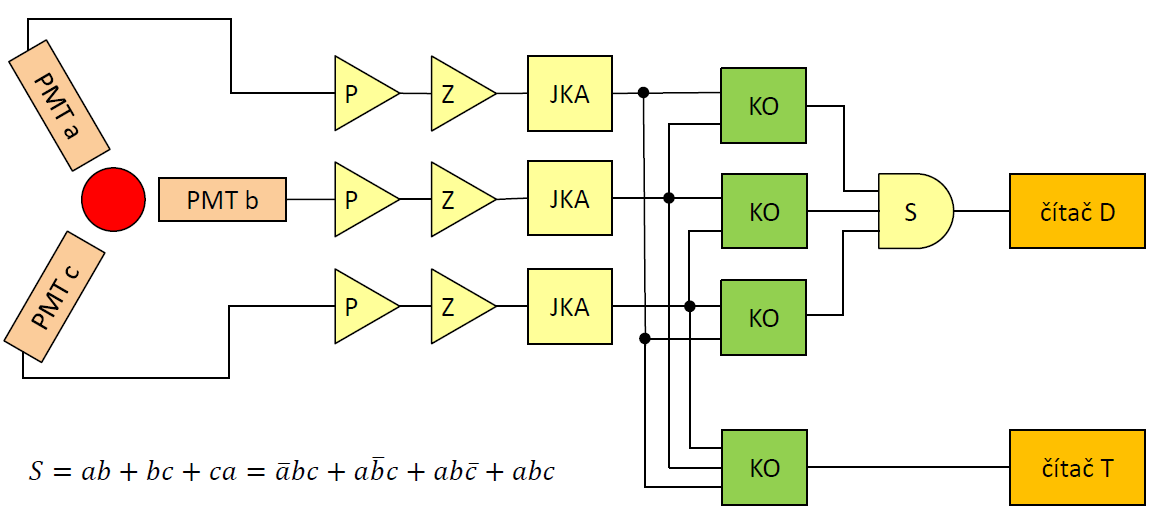
\includegraphics[width=1\linewidth]{img/tdcr.png}
    \caption{TDCR}
\end{figure}
